\section{Methods} \label{sec:methods}

In this section, we address the problems inherent in both the Hald and Modified Hald models.  Our approach builds on these models by introducing a fully joint model for both source and human case 
sampling.  This allows us to integrate over uncertainty in the source sampling process, estimating both the prevalence of contaminated source samples and the relative prevalence of each identified 
subtype, without resorting to an approximate marginal probability distribution on $\bm{r}$.  Furthermore, we introduce non-parametric clustering of pathogen types using a Dirichlet process model on 
the type effect vector $\bm{q}$, providing an automatic data-driven way of reducing the dimensionality of $\bm{q}$ to aid model identifiability.  We are able, therefore, to circumvent the Hald model 
requirement for heuristically grouping pathogen types (Section \ref{sec:hald}), as well as avoiding an arbitrarily strong prior distribution on a random effect precision parameter as required by 
the Modified Hald model (Section \ref{sec:modifiedHald}).  

\subsection{Model} \label{sec:model}

As with the Hald and Modified Hald models, the number of human cases $y_i$ identified by isolation of subtype $i$ is assumed to be Poisson distributed so that
\begin{equation}\label{eq:likelihood}
y_{i}\sim \textsf{Poisson}(\lambda_{i})
\end{equation}

The mean intensity $\lambda_{i}$ is a linear combination of type and source-specific effects such that
\begin{equation}
\lambda_i = q_{i} \sum_{j=1}^{m} a_{j} p_{ij}
\end{equation}
where $a_j$ represents the source effect, $p_{ij}$ the absolute prevalence of subtype $i$ in samples from source $j$, and $q_{i}$ is the type effect for subtype $i$.

For each source $j=1,\dots,m$, we model the number of positive samples $x_{ij}$ identified as type $i=1,\dots,n$ as
\begin{equation}
\bm{x}_j \sim \mbox{Multinomial}(n_j, \bm{r}_j)
\end{equation}
where $\bm{x}_j$ denotes the vector of type-counts in source $j$, $n_j$ denotes the number of positive samples obtained from source $j$, and $\bm{r}_j$ denotes a vector of relative prevalences of  
isolate types in source $j$.  The advantage of this model is that it automatically places the constraint $\sum_{i=1}^{n} r_{ij} = 1$,  avoiding the approximation made in \citet{MulJonNob09} where 
independent Beta-distributed priors were assigned marginally to components of $\bm{r}_j$ .  The source case model is then coupled to the human case model through the simple relationship 
\begin{equation}
p_{ij} = r_{ij}\pi_j
\end{equation}
where $\pi_j$ is the prevalence of any isolate in source $j$.

We note that in principle, a Beta distribution could be used to model $\pi_j$, arising as the conjugate posterior distribution of a Binomial sampling model for $x_j$ positive samples from $n_j$ tested, 
and a Beta prior on $\pi_j$.  However, since within a particular source the number of positive and negative samples are typically high, we choose to fix the source prevalences at their point estimates 
($\pi_j=x_j/n_j$). 


The type effects, $\bm{q}$ are drawn from a Dirichlet Process
\begin{equation}
q_i \sim \mbox{DP}\left( \alpha_q, Q_0 \right). \label{eq:qDP}
\end{equation}
The Dirichlet Process is a random probability measure defined by a base distribution $Q_0$ and a concentration parameter $\alpha_q$ \citep{Fer73}. The base distribution constitutes a prior 
distribution in the values of each element of the type effects $\mathbf{q}$ whilst the concentration parameter encodes prior information on the number of groups $K$ to which each subtype $i$ is 
assigned. For small values of $\alpha_q$, samples from the DP are likely to have a small number of atomic measures with large weights. For large values, most samples are likely to be distinct, and 
hence, concentrated on $Q_{0}$. A value of 1 implies that, \emph{a priori}, two randomly selected types have probability 0.5 of belonging to the same cluster \citep{GelCarSte13}.


%\noindent\begin{minipage}{\linewidth}
\begin{knitrout}
\definecolor{shadecolor}{rgb}{0.969, 0.969, 0.969}\color{fgcolor}\begin{figure}[H]

{\centering 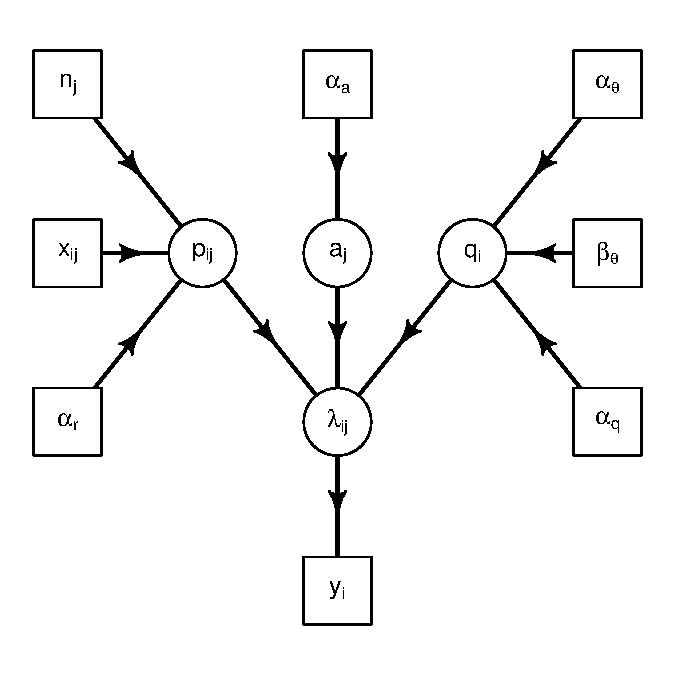
\includegraphics[width=\maxwidth]{DAG-1} 

}

\caption{Directed acyclic graph of the source attribution model. See Table \ref{table_params} for a concise description of the parameters.}
\label{fig:DAG}
\end{figure}
\end{knitrout}

\begin{table}[H] %%[!htb] This forces latex to ignore the float placement rules
\caption{Description and definition of parameters used in our model.}\label{table_params}
\setlength{\tabcolsep}{4pt}
\bigskip{}
\centering
\label{table:HaldModelParams}
\begin{tabular}{lll}
\multicolumn{1}{l}{\textbf{Parameter}} & \multicolumn{1}{l}{\textbf{Description}} & \multicolumn{1}{l}{\textbf{Estimation}}\\
$\lambda_{ij}$ & Number of human cases from type $i$, source $j$ & $\lambda_{ij}=a_{j}\cdot q_{k(i)}\cdot r_{ij}\cdot \pi_{j}$\\
$\lambda_{i}$ & Number of human cases from type $i$ & $\lambda_{i}=\sum_{j=1}^{m}\lambda_{ij}$\\
$\lambda_{j}$ & Number of human cases from source $j$ & $\lambda_{j}=\sum_{i=1}^{n}\lambda_{ij}$\\
$y_{i}$ & Number of human cases from type $i$ & $y_{i}\sim \textsf{Poisson}(\lambda_{i})$\\
&&\\
$x_{ij}$ & Number of positive samples (that were & Data\\
& successfully MLST typed) from source $j$, type $i$ & \\
$h_{ij}$  & Number of positive samples (PCR) that & Data\\
& could not be MLST typed. & \\
$n_{j}$ & Total number of samples from source $j$ & Data\\
 &&\\
$\pi_{j}$ & Prevalence of contamination for each source & $\sum_{i=1}^{I}(x_{ij}+h_{ij})/n_{j}$\\
$r_{ij}$ & Relative occurrence of type $i$ on source $j$ & $\mathbf{r}_j\sim \textsf{Dirichlet}(\alpha_r)$\\
& & or $x_{ij}/\sum_{i=1}^{n}x_{ij}$\\
$p_{ij}$ & Absolute prevalence of type $i$ in source $j$ & $r_{ij}\cdot \pi_{j}$\\
$a_{j}$ & Unknown source effect for source $j$ & $\mathbf{a}\sim \textsf{Dirichlet}(\alpha_a)$\\
$q_{i}$ & Unknown type effect for type $i$ in group $k$,& $\mathbf{q}\sim \textsf{DP}(\textsf{Gamma}(\alpha_{\theta}, \beta_{\theta}), \alpha_q)$\\
 & where group $k$ has an unknown value $\theta_k$ &\\
\end{tabular}\\
\end{table}
%\end{minipage}

\subsection{Model extensions} 

The models can further be extended to incorporate a time and location dependence into the model allowing different rates over time and in different locations (such as urban vs rural cases). Let $
\lambda_{ijtl}$ be the expected number of infections of sequence type $i$ attributable to source $j$ at time $t$ with location $l$. Then the observed human counts from a particular type $i$ during that 
time period in a particular location $y_{itl}$ is given by
$$
y_{itl}\sim \textsf{Poisson}(\sum_{j=1}^{m}\lambda_{ijtl})
$$
where
\begin{equation}
\lambda_{ijtl} = q_i a_{jtl} r_{ijt} \pi_{jt}.
\end{equation}

Note that type effects $\bm{q}$ are assumed to be constant over all times and locations, and source effects $\bm{a}$ are allowed to vary between times and locations.  Importantly, the source 
sampling information ($\bm{r}_t$ and $\bm{\pi}_t$) are allowed to vary by time only.  This is because of the the nature of food source sampling at the point of sale, where food retailers move 
packaged meat long distances from the farm to retail store.  This is implemented in \pkg{sourceR} as shown in Section \ref{sim_study_section}.

